% !TEX encoding = UTF-8
% !TEX TS-program = pdflatex
% !TEX root = ../tesi.tex
% !TEX spellcheck = it-IT

%************************************************
\chapter{Classificazione}
\label{cap:ctbnc}
%************************************************
La classificazione è un argomento centrale nei campi di ricerca relativi all'\keyword{apprendimento automatico} (anche detto \keyword{machine learning}) e l'analisi dei dati. In generale, essa consiste nel processo di assegnare una \emph{classe} (\ie{} un'etichetta) a delle istanze descritte da un insieme di attributi. Si parla di \emph{classificazione \keywordsub[classificazione]{supervisionata}} quando è necessario indurre un \keywordsub[classificazione]{classificatore} a partire da un insieme di dati composto da istanze già etichettate e utilizzare tale classificatore per classificare nuove istanze di dati.

In questo capitolo viene quindi introdotta una classe di modelli, che prende il nome di \acf{CTBNC}, il cui scopo è la \emph{classificazione supervisionata} di traiettorie multivariate di variabili discrete a \emph{tempo continuo}. Si descrivono due istanze di tale classe: i classificatori \acf{CTNB} e i classificatori \acf{CTTANB}.

Mentre nella \autoref{sec:learning-ctbnc} si affronta il processo di \emph{\keywordsub[classificazione]{apprendimento}} in caso di \emph{dati completi} dei \acs{CTBNC}, nella \autoref{sec:inference-ctbnc}, si presenta un algoritmo di \emph{\keywordsub[classificazione]{inferenza} esatta} per la classe dei \acs{CTBNC}.

\section{Modello}\label{sec:ctbnc-model}
Al fine di risolvere il succitato problema della classificazione sono stati proposti numerosi approcci. Ad esempio \lwcase \nb{} \class{}, un classificatore semplice ma robusto proposto da~\citet{DudaHart1973}; rivelatosi essere uno fra i classificatori più performanti~\citep{Langley1992}. Esso apprende dai dati la probabilità condizionale di ogni attributo $\setel{A}_i$ data la classe $\setel{C}$. La classificazione di nuove istanze dei dati è effettuata applicando la \emph{regola di Bayes} al fine di calcolare la probabilità della classe $\setel{C}$ data l'istanziazione di $\setel{A}_i,\,\dotsc\,,\setel{A}_N$ e scegliendo quella con la maggiore probabilità a posteriori. Questo calcolo è reso possibile da un'assunzione forte: tutti gli attributi $\setel{A}_i$ sono \emph{condizionalmente indipendenti} (si veda la \autoref{defn:ic}) tra di loro data evidenza sulla classe $\setel{C}$.

Poiché tale assunzione è chiaramente irreale,~\citet{Friedman1997} ha investigato come migliorare ulteriormente le prestazioni del \lwcase \nb{} \class{} evitando assunzioni di indipendenza non giustificate dai dati. A tal fine~\citet{Friedman1997}, generalizzando il \lwcase \nb{} \class{}, ha proposto una classe di modelli di \emph{classificazione supervisionata}, chiamata \acf{BNC} (di cui fa parte il \acf{TAN} \class{}, ad esempio) che ereditano dalla teoria delle \acl{BN} (si rimanda alla \autoref{defn:bn} per maggiori dettagli) una rappresentazione fattorizzata delle distribuzioni di probabilità dei nodi attributo e rappresentano esplicitamente le indipendenze condizionali fra essi.

Seguendo le stesse motivazioni, in ~\citet{Stella2012} viene formalizzata una classe di modelli di \emph{classificazione supervisionata}, chiamati \acf{CTBNC}, derivata dalle \acs{CTBN} (si veda \autoref{defn:ctbn}).

Di seguito si definiscono quindi i \acl{CTBNC} e due istanze di classificatori appartenenti a tale classe: il \acf{CTNBC} e il \acf{CTTANBC}.

Un \acl{CTBNC} estende una \acs{CTBN} tramite l'aggiunta di un nodo associato alla variabile classe $\setel{Y}$. Si ricorda, dalla \autoref{defn:ctbn}, che una \acs{CTBN} rappresenta l'evoluzione nel tempo continuo di una \pv{} $\set{X}$ (\ie{} insieme composto da $N$ \mprocess{}, si veda la \autoref{defn:pv}).

Di seguito si dà la definizione di questa nuova classe di modelli di \emph{classificazione supervisionata}.
\begin{definizione}[\acl{CTBNC}]\label{defn:ctbnc}
Un \acf{CTBNC} è composto da una coppia $\conceptsym{C}=(\conceptsym{N}\,,\,\set{P}(\setel{Y}))$ dove:
\begin{itemize}
    \item $\conceptsym{N}$ è una \acs{CTBN} con nodi attributo $\setel{X_1}\,,\,\setel{X_2}\,,\,\dotsc\,,\,\setel{X_N}$
    \item $\setel{Y}$ è il nodo classe con valori $val(\setel{Y})=\{\,\vectel{y_1}\,,\,\dotsc\,,\,\vectel{y_K}\,\}$ e probabilità marginale $\set{P}(\setel{Y})$.
\end{itemize}
E inoltre il grafo su $\conceptsym{N}$ (\ie{} il grafo $\conceptsym{G}$, si veda la \autoref{defn:ctbn}) rispetta le seguenti condizioni:
\begin{itemize}
    \item $\conceptsym{G}$ è un grafo connesso\footnote{Il grafo $\conceptsym{G} = (\setel{V}, \setel{E})$ è detto \emph{connesso} se $\forall \: (\setel{u}\,,\,\setel{v}) \in \setel{V}$ esiste un cammino che collega $\setel{u}$ a $\setel{v}$.}
    \item $Pa(\setel{Y})=\{\,\}$, \ie{} la variabile casuale $\setel{Y}$ è associata a un nodo radice\footnote{In un grafo un nodo è detto \emph{radice} qualora esso non abbia alcun genitore.}
    \item il nodo $\setel{Y}$ è indipendente dal tempo ed è specificato solo ed esclusivamente dalla sua probabilità marginale $\set{P}(\setel{Y})$.
\end{itemize}
\end{definizione}
A supporto della \autoref{defn:ctbnc}, la figura~\vref{fig:ctbnc-example} fornisce un'istanza di \acs{CTBNC} composta dai nodi attributi $\setel{X_1},\setel{X_2},\setel{X_3},\setel{X_4},\setel{X_5}$ e dal nodo classe $\setel{Y}$ (nodo radice). Si osservi come tale istanza contenga dei cicli, uno riguardante i nodi $\setel{X_2},\setel{X_4},\setel{X_5},\setel{X_3}$ e l'altro riguardante i nodi $\setel{X_1},\setel{X_3}$. Si fa notare che gli archi della rete $\conceptsym{N}$ rappresentano le dipendenze causali nel tempo.

\newpage

\begin{figure}
\centering
\includegraphics[width=0.8\columnwidth]{ctbnc}
\caption[Un esempio di \acs{CTBNC}]{Un esempio di \acf{CTBNC} con cinque nodi attributo, $\setel{X}_1\,,\,\dotsc\,,\,\setel{X}_5$, e un nodo classe, $\setel{Y}$.}
\label{fig:ctbnc-example}
\end{figure}

Parallelamente a quanto fatto in~\citet{Langley1992}, si presentano ora due istanze particolari di \acl{CTBNC}.

\begin{definizione}[\acl{CTNBC}]\label{defn:ctnbc}
Un \acf{CTNBC} è un \acl{CTBNC} $\conceptsym{C}=(\conceptsym{N}\,,\,\set{P}(\setel{Y}))$ caratterizzato dal fatto che ogni nodo attributo ha un solo genitore, il nodo classe $\setel{Y}$. Risulta quindi che:
\[
Pa(\setel{X}_i)=\{\,\setel{Y}\,\} \quad \forall \; \setel{X}_i \in \conceptsym{G}\text{.}
\]
\end{definizione}
Come mostrato dalla figura~\vref{fig:ctnbc}, un \acs{CTNBC} possiede un nodo radice, associato alla variabile casuale $\setel{Y}$, che è l'unico genitore di tutti i restanti nodi $\setel{X}_i$ (con $i=1,2,\,\dotsc\,,N$) che lo compongono. Si osservi come la rete di un \acs{CTNBC} rappresenti l'assunzione di \emph{indipendenza condizionale} di ogni nodo attributo dagli altri, data evidenza sulla variabile classe $Y$.

\begin{figure}[b]
\centering
\includegraphics[width=0.9\columnwidth]{ctnb}
\caption[Un \acs{CTNBC}]{Un \acf{CTNBC}.}
\label{fig:ctnbc}
\end{figure}

\begin{definizione}[\acl{CTTANBC}]\label{defn:cttanbc}
Un \acf{CTTANBC} è un \acl{CTBNC} $\conceptsym{C}=(\conceptsym{N}\,,\,\set{P}(\setel{Y}))$ che rispetta i seguenti vincoli:
\begin{itemize}
    \item $\setel{Y} \in Pa(\setel{X}_i)$ con $i=1,2,\,\dotsc\,,N$
    \item i nodi attributo $\setel{X}_i$, $i=1,2,\,\dotsc\,,N$, formano un albero:
    \[
    \exists \; j \; : \quad |Pa(\setel{X}_j)|=1 \quad \text{mentre per} \quad i \neq j \; : \quad |Pa(\setel{X}_i)|=2\text{.}
    \]
\end{itemize}
\end{definizione}
Come mostrato dalla figura~\ref{fig:cttanbc} un classificatore \acs{CTTANB} è un estensione del classificatore \acs{CTNB}: tutti i nodi attributo della rete $\conceptsym{N}$ sono vincolati ad avere come genitore, oltre al nodo radice, al massimo un altro nodo attributo. Ciò comporta che tutti i nodi attributo facciano parte del \emph{Markov blanket}\cref{note:markov-blanket} del nodo radice associato con la variabile classe $\setel{Y}$.

\begin{figure}
\centering
\includegraphics[width=0.9\columnwidth]{cttanb}
\caption[Un \acs{CTTANBC}]{Un \acf{CTTANBC}: qualora la variabile classe $\setel{Y}$ venga rimossa, le variabili rimanenti formano un albero.}
\label{fig:cttanbc}
\end{figure}

\section{Apprendimento}\label{sec:learning-ctbnc}
In questa sezione si affronta il problema dell'apprendimento (da \emph{dati completi}) dei \acs{CTBNC}.

Per definizione (si veda \ref{defn:ctbnc}) i \acs{CTBNC} sono basati sul modello delle \acs{CTBN}, rappresentano perciò un insieme di modelli di probabilità locali (relativi alle variabili casuali) esprimibili in termini di statistiche sufficienti (per maggiori dettagli relativi a questo aspetto si rimanda alla \autoref{sec:ctbn-apprendimento}). Ne deriva che il problema dell'apprendimento di un classificatore \acs{CTBN} si riduce alla computazione delle \keyword{statistiche sufficienti} dei suoi nodi attributo, da cui è successivamente possibile (nonché semplice) stimare i parametri (argomento trattato in dettaglio nella \autoref{sec:ctbn-params}) delle \cim{} (\acs{CIM}).

Di conseguenza, per l'apprendimento di un \acs{CTNBC} è richiesto uno sforzo computazionale minimo. Per l'apprendimento di un \acs{CTTANBC}, poiché questo modello prevede archi anche fra i nodi attributo, è invece richiesto uno sforzo computazionale leggermente maggiore~\citep{Stella2012}.

Si presenta di seguito l'\autoref{lst:ctnbc-learning} relativo all'apprendimento di un classificatore \acs{CTNB} (\autoref{defn:ctnbc}).

Esso richiede in input un \emph{dataset completo} $\conceptsym{D}=\{\,\delta_1\,,\,\dotsc\,,\,\delta_h\,\}$, il corrispettivo insieme delle classi $\{\setel{y}_1\,,\,\setel{y}_2\,,\,\dotsc\,,\,\setel{y}_h\}$, con $\setel{y}_i \in val(\setel{Y})$, e il grafo $\conceptsym{G}$ di una \acs{CTBN} $\conceptsym{N}$ (rispettivamente chiamati \lstinline[]|data|, \lstinline[]|classes| e \lstinline[]|graph| nella firma della funzione \lstinline[]|ctnbclearn|).

Per completezza si osservi (in base alla \autoref{defn:dataset-completo}) che ogni $\delta_i$ (con $i=1\,,\,\dotsc\,,\,h$) è un flusso di evidenze $\evidencestream{J_i}$ (a tal riguardo si veda la \autoref{defn:j-evidence-stream}).

Il risultato dell'applicazione dell'\autoref{lst:ctnbc-learning} è un \acl{CTNBC} $\conceptsym{C}=(\conceptsym{N}\,,\,\set{P}(\setel{Y}))$.
\begin{lstlisting}[caption=Apprendimento di un classificatore \acs{CTNB}, label=lst:ctnbc-learning]
function ctnbclearn(data, classes, graph) {
    <ls>\label{lst:start-prior-computation}<le>var h = len(data)
    var klass = unique(classes)
    var nk = len(class)
    var priors[nk]
    for (i in index(data)) {
        var k = index(classes[i])
        priors[k] = priors[k] + (1 / h)
    }<ls>\label{lst:end-prior-computation}<le>
    <ls>\label{lst:start-ss-computation}<le>var m(), t()
    for (i in index(data)) {
        var y = classes[i]
        var j = 1
        while (<ls>$t_j \leq T_i$<le>) {
            for (n in index(graph.nodes)) {
                m(<ls>$\setel{x}_n^j$<le>, <ls>$\setel{x}_n^{j+1}$<le>, y) = m(<ls>$\setel{x}_n^j$<le>, <ls>$\setel{x}_n^{j+1}$<le>, y) + 1
                t(<ls>$\setel{x}_n^j$<le>, y) = t(<ls>$\setel{x}_n^j$<le>, y) + <ls>$(t_j - t_{j-1})$<le>
            }
            j = j + 1
        }
    }<ls>\label{lst:end-ss-computation}<le>
    <ls>\label{lst:start-params-computation}<le>var q(), thet()
    foreach (y in klass) {
        for (n in index(graph.nodes)) {
            for (<ls>$\setel{x}_n$<le> in <ls>$val(\setel{X}_n)$<le>) {
                var mm(<ls>$\setel{x}_n$<le>, y) = <ls>$\sum_{\setel{x}_n^{\prime}\neq\setel{x}_n}$<le> m(<ls>$\setel{x}_n$<le>, <ls>$\setel{x}_n^{\prime}$<le>, y)
                q(<ls>$\setel{x}_n$<le>, y) = mm(<ls>$\setel{x}_n$<le>, y) / t(<ls>$\setel{x}_n$<le>, y)
                thet(<ls>$\setel{x}_n$<le>, y) = m(<ls>$\setel{x}_n$<le>, <ls>$\setel{x}_n^{\prime}$<le>, y) / mm(<ls>$\setel{x}_n$<le>, y)
            }
        }
    }<ls>\label{lst:end-params-computation}<le>
    var ctbn = new ctbn(graph, q, thet)
    return (priors, ctbn)
}
\end{lstlisting}

L'algoritmo (\ref{lst:ctnbc-learning}) di apprendimento appena presentato consiste nella stima delle \cim{} (\acs{CIM}) di ogni variabile casuale di $\conceptsym{N}$ per ogni classe $\setel{y}_i \in \setel{Y}$. Più in dettaglio, esso è composto da tre fasi consecutive:
\begin{enumerate}
    \item da \autoref{lst:start-prior-computation} a \autoref{lst:end-prior-computation} viene calcolata la \emph{probabilità a priori} della variabile classe $\setel{Y}$ in base alla frequenza di ogni sua istanziazione $\setel{y}_i \in\setel{Y}$ in $\conceptsym{D}$
    \item da \autoref{lst:start-ss-computation} a \autoref{lst:end-ss-computation} vengono calcolate le \emph{statistiche sufficienti} di ogni nodo attributo $\setel{X}_i$, con $i=1,2,\,\dotsc\,,N$, sull'insieme di dati di apprendimento (anche detto \emph{\keywordsub[classificazione]{training set}}) $\conceptsym{D}$
    \item da \autoref{lst:start-params-computation} a \autoref{lst:end-params-computation} vengono infine stimati, a partire dalle statistiche sufficienti, i \emph{parametri \acl{MLE}} (\acs{MLE}).
\end{enumerate}
Si osservi che, poiché il processo di apprendimento è eseguito su un classificatore \acs{CTNB}, l'algoritmo condiziona sia il calcolo delle statistiche sufficienti (\ie{} variabili \lstinline[]|t| e \lstinline[]|m|) che la stima dei parametri (\ie{} variabili \lstinline[]|q| e \lstinline[]|thet|) di ogni nodo attributo $\setel{X}_i$ solo ed esclusivamente al valore della variabile classe $\setel{Y}$ (\ie{} variabile \lstinline[]|y|). Questa semplificazione è dovuta al vincolo che caratterizza i classificatori \acs{CTNB}: ogni nodo attributo $\setel{X}_i$ deve avere un solo genitore, il nodo associato alla variabile classe $\setel{Y}$ (si veda la \autoref{defn:ctnbc}).

Come anticipato, al costo di un leggero incremento di complessità computazionale, è possibile estendere l'\autoref{lst:ctnbc-learning} al fine di creare un algoritmo di apprendimento generale che apprenda un qualsiasi classificatore \acs{CTBN}. Affinché tale obiettivo sia raggiunto è necessario rimuovere il succitato vincolo sull'insieme dei genitori di ogni nodo attributo. Mentre il calcolo della probabilità a priori della variabile classe $\setel{Y}$ non varia, il calcolo delle statistiche sufficienti e la stima dei parametri, invece, necessitano di tale generalizzazione.

Nello specifico:
\begin{enumerate}
    \item il calcolo delle statistiche sufficienti di ogni nodo attributo $\setel{X}_i$ va condizionato all'istanziazione attuale (\ie{} al tempo $j$) del suo insieme di nodi genitori $Pa(\setel{X}_i)$; perciò a \autoref{lst:general-ss-computation} dell'\autoref{lst:ctbnc-learning} si prende in considerazione tale valore (\ie{} variabile \lstinline[]|p|)
    \item la stima dei parametri \acl{MLE} (\acs{MLE}) di ogni noto attributo $\setel{X}_i$ va eseguita in base a ogni istanziazione del suo insieme di nodi genitori $Pa(\setel{X}_i)$; perciò a \autoref{lst:general-params-computation} si itera in base a ogni valore (\ie{} variabile \lstinline[]|p|) assunto da $Pa(\setel{X}_i)$ (\ie{} $val(Pa(\setel{X}_i))$) mentre l'iterazione per classe non è più coerente e di conseguenza rimossa.
\end{enumerate}
Si riporta di seguito l'\autoref{lst:ctbnc-learning}, il quale include le succitate modifiche finalizzate alla creazione di un algoritmo di apprendimento generale per i \acs{CTBNC}.
\begin{lstlisting}[caption=Apprendimento di un classificatore \acs{CTBN}, label=lst:ctbnc-learning]
function learn(data, classes, graph) {
    var h = len(data)
    var klass = unique(classes)
    var nk = len(class)
    var priors[nk]
    for (i in index(data)) {
        var k = index(classes[i])
        priors[k] = priors[k] + (1 / h)
    }
    var m(), t()
    foreach (i in index(data)) {
        var j = 1
        while (<ls>$t_j \leq T_i$<le>) {
            foreach (n in index(graph.nodes)) {
                var p = <ls>$val^j(Pa(\setel{X}_n))$\label{lst:general-ss-computation}<le>
                m(<ls>$\setel{x}_n^j$<le>, <ls>$\setel{x}_n^{j+1}$<le>, p) = m(<ls>$\setel{x}_n^j$<le>, <ls>$\setel{x}_n^{j+1}$<le>, p) + 1
                t(<ls>$\setel{x}_n^j$<le>, p) = t(<ls>$\setel{x}_n^j$<le>, p) + <ls>$(t_j - t_{j-1})$<le>
            }
            j = j + 1
        }
    }
    var q(), thet()
    foreach (n in index(graph.nodes)) {
        for (<ls>$\setel{x}_n$<le> in <ls>$val(\setel{X}_n)$<le>) {
            foreach (p in <ls>$val(Pa(\setel{X}_n))$\label{lst:general-params-computation}<le>) {
                var mm(<ls>$\setel{x}_n$<le>, p) = <ls>$\sum_{\setel{x}_n^{\prime}\neq\setel{x}_n}$<le> m(<ls>$\setel{x}_n$<le>, <ls>$\setel{x}_n^{\prime}$<le>, p)
                q(<ls>$\setel{x}_n$<le>, p) = mm(<ls>$\setel{x}_n$<le>, p) / t(<ls>$\setel{x}_n$<le>, p)
                thet(<ls>$\setel{x}_n$<le>, p) = m(<ls>$\setel{x}_n$<le>, <ls>$\setel{x}_n^{\prime}$<le>, p) / mm(<ls>$\setel{x}_n$<le>, p)
            }
        }
    }
    var ctbn = new ctbn(graph, q, thet)
    return (priors, ctbn)
}
\end{lstlisting}

\section{Inferenza}\label{sec:inference-ctbnc}
In questa sezione si affronta il problema della \emph{\keyword{classificazione}} di un \emph{flusso di evidenze completamente osservato}, indicato con $\evidencestream{J}$ (si veda la \autoref{defn:j-evidence-stream}), rispetto a un classificatore \acs{CTBN} (\acs{CTBNC}). L'argomento di questa sezione è quindi il processo di \emph{classificazione supervisionata} (\ie{} è necessario un \acs{CTBNC} appreso da un \emph{training set}), di cui si presentano in primis le basi teoriche e successivamente l'implementazione algoritmica che ne consegue.

Il processo di classificazione di un flusso di evidenze è effettuato in base alla regola \emph{\acl{MAP}}\footnote{\ACF{MAP}, \omissis} (\acs{MAP})~\citep[si veda][]{Stella2012}: un flusso di evidenze completamente osservato viene classificato assegnandogli la classe la cui probabilità a posteriori (rispetto al flusso di evidenze stesso) è massima. A tale scopo è necessario calcolare la probabilità a posteriori della variabile classe $\setel{Y}$ del \acs{CTBNC}, rispetto al flusso di evidenze in input, per tutti i suoi possibili stati (\ie{} classi, o etichette).

Il classificatore \acs{CTBN} classifica quindi il flusso di evidenze massimizzando la seguente probabilità a posteriori, ricavata applicando la \emph{\keywordsub[classificazione]{regola di Bayes}}:
\begin{equation}\label{eq:ctbnc-inference-1}
P(\setel{Y}\,\arrowvert\,\evidencestream{J})=\frac{P(\evidencestream{J}\,\arrowvert\,\setel{Y})\:P(\setel{Y})}{P(\evidencestream{J})}\text{.}
\end{equation}
Si specifica di seguito la semantica dei componenti dell'\autoref{eq:ctbnc-inference-1}:
\begin{itemize}
\item la probabilità marginale associata alla variabile classe $\setel{Y}$ \[P(\setel{Y})\]
\item la probabilità del flusso di evidenze \[P(\evidencestream{J})\]
\item la likelihood\cref{note:likelihood} del flusso di evidenze dato il valore della variabile classe, a cui ci si riferisce nel prosieguo usando l'espressione \emph{\virgolette{\keywordsub[classificazione]{likelihood temporale}}} \[P(\evidencestream{J}\,\arrowvert\,\setel{Y})\text{.}\]
\end{itemize}
La probabilità del flusso di evidenze, similmente a quanto accade per i \acs{BNC}~\citep{Friedman1997}, non è richiesta per l'implementazione della regola \acs{MAP}, perciò è possibile ometterla e riscrivere la precedente equazione sotto forma di relazione proporzionale:
\begin{equation}\label{eq:ctbnc-inference-2}
P(\setel{Y}\,\arrowvert\,\evidencestream{J}) \propto P(\evidencestream{J}\,\arrowvert\,\setel{Y})\:P(\setel{Y})\text{.}
\end{equation}
Il primo termine dell'\autoref{eq:ctbnc-inference-2}, cioè la \emph{\keywordsub[classificazione]{likelihood temporale}}, è invece fondamentale per la classificazione tramite regola \acs{MAP} ed è possibile riformularlo nel seguente modo:
\begin{equation}\label{eq:ctbnc-inference-3}
P(\evidencestream{J}\,\arrowvert\,\setel{Y})=\prod_{j=1}^{J} P(\set{x}^j\,\arrowvert\,\setel{Y})\:P(\set{x}^{j+1}\,\arrowvert\,\set{x}^j,\setel{Y})\text{,}
\end{equation}
dove:
\begin{itemize}
    \item $P(\set{x}^j\,\arrowvert\,\setel{Y})$ rappresenta la probabilità che il \emph{\keywordsub[classificazione]{vettore aleatorio}}\footnote{\label{note:vettore-aleatorio}Un \emph{vettore aleatorio} $\set{X}=(\setel{X}_1,\setel{X}_2,\,\dotsc\,,\setel{X}_n)$ è una $n$\emph{-upla} (composta da $n$ variabili casuali) i cui elementi sono dati da numeri aleatori.} $\set{X}$ resti nello stato $\set{x}^j$ durante l'intervallo temporale $[\,t_{j-1},\,t_j)$ data evidenza sulla variabile classe $\setel{Y}$
    \item $P(\set{x}^{j+1}\,\arrowvert\,\set{x}^j,\setel{Y})$ rappresenta la probabilità che in $\set{X}$ si verifichi una transizione da $\set{x}^j$ a $\set{x}^{j+1}$ all'istante di tempo $t_j$ data evidenza sulla variabile classe $\setel{Y}$.
\end{itemize}
Inoltre, al fine di assicurare la consistenza dell'\autoref{eq:ctbnc-inference-3} si assume che $P(\set{x}^{J+1}\,\arrowvert\,\set{x}^J,\setel{Y})=1$.

Il passo successivo consiste nel calcolo dei due termini da cui è composta l'\autoref{eq:ctbnc-inference-3}. A tal fine si utilizzano le distribuzioni di probabilità locali associate ad ogni nodo del \acs{CTBN} su cui è costruito il classificatore. Come già descritto nella \autoref{sec:mps}, tali modelli di probabilità sono espressi tramite le \cim{} e quindi tramite i parametri $q$ e $\theta$.

In tale contesto è quindi possibile calcolare il termine $P(\set{x}^j\,\arrowvert\,\setel{Y})$ come segue:
\begin{equation}\label{eq:ctbnc-inference-4}
P(\set{x}^j\,\arrowvert\,\setel{Y})=\prod_{n=1}^N exp\Big(-q_{\setel{x}_n^j}^{pa_j(\setel{x}_n)}\:(t_j - t_{j-1})\Big)\text{,}
\end{equation}
dove $q_{\setel{x}_n^j}^{pa_j(\setel{x}_n)}$ è il valore del parametro della \emph{distribuzione esponenziale} quando la variabile casuale $\setel{X}_n$ è nello stato $\setel{x}_n$ durante il $j$-esimo intervallo temporale $[\,t_{j-1},\,t_j)$ e contemporaneamente l'istanziazione dei genitori di $\setel{X}_n$ è $pa_j(\setel{x}_n)$.

Ugualmente, il termine $P(\set{x}^{j+1}\,\arrowvert\,\set{x}^j,\setel{Y})$ è così calcolabile:
\begin{equation}\label{eq:ctbnc-inference-5}
P(\set{x}^{j+1}\,\arrowvert\,\set{x}^j,\setel{Y})=\prod_{n=1}^N P(\setel{x}_n^{j+1}\,\arrowvert\,\setel{x}_n^j,\setel{Y})\text{,}
\end{equation}
dove
\begin{equation}\label{eq:ctbnc-inference-6}
P(\setel{x}_n^{j+1}\,\arrowvert\,\setel{x}_n^j,\setel{Y})=
\begin{cases}
q_{\setel{x}_n^j\setel{x}_n^{j+1}}^{pa_j(\setel{x})}, & \text{se } \setel{x}_n^j \neq \setel{x}_n^{j+1} \\
1, & \text{altrimenti}
\end{cases}\text{.}
\end{equation}
Il termine $P(\setel{x}_n^{j+1}\,\arrowvert\,\setel{x}_n^j,\setel{Y})$ rappresenta la probabilità che nel vettore aleatorio $\set{X}$ si verifichi una transizione dallo stato $\set{x}^j$ allo $\set{x}^{j+1}$, dato il valore della variabile classe $\setel{Y}$.

%TODO: sta roba di una transizione alla volta va detta nel capitolo 2, in "rappresentazione", o simili, poi ripresa qui (e linkata)
Poiché il modello \acs{CTBN} implica che, ad ogni istante $t_j$, solo un componente $\setel{X}_n$ del vettore aleatorio $\set{X}$ può essere soggetto a transizione, allora $P(\setel{x}_n^{j+1}\,\arrowvert\,\setel{x}_n^j,\setel{Y})$ rappresenta la probabilità che la variabile casuale $\setel{X}_n$ effettui una transizione da $\setel{x}_n^j$ a $\setel{x}_n^{j+1}$ mentre tutti gli altri componenti del \keywordsub[classificazione]{vettore aleatorio} $\set{X}$ (\ie{} $\setel{X}_i$ con $i \neq n$) non cambiano il proprio stato.

Perciò, come specificato dall'\autoref{eq:ctbnc-inference-6}, nel caso in cui avvenga un cambio di stato di $\setel{X}_n$, il termine $P(\setel{x}_n^{j+1}\,\arrowvert\,\setel{x}_n^j,\setel{Y})$ equivale alla quantità $q_{\setel{x}_n^j\setel{x}_n^{j+1}}^{pa_j(\setel{x})}$, ricavata dall'\autoref{eq:ctbn-params-rel}, moltiplicando la \emph{\virgolette{probabilità istantanea}} di transizione da $\setel{x}_n^j$ a $\setel{x}_n^{j+1}$ e il tempo atteso di transizione uscente dallo stato $\setel{x}_n^j$. Tale quantità rappresenta il parametro associato alla transizione da $\setel{x}_n^j$, stato in cui la variabile casuale $\setel{X}_n$ si trovava durante il $j$-esimo intervallo temporale $[\,t_{j-1},\,t_j)$, a $\setel{x}_n^{j+1}$, stato in cui $\setel{X}_n$ si troverà durante il successivo intervallo temporale $[\,t_j,\,t_{j+1})$; data l'istanziazione $pa_j(\setel{x}_n)$ dei genitori di $\setel{X}_n$ durante il $j$-esimo intervallo temporale.

Combinando l'\autoref{eq:ctbnc-inference-4} e l'\autoref{eq:ctbnc-inference-5} si ottiene:
\footnotesize
\begin{equation}\label{eq:ctbnc-inference-7}
P(\set{x}^j\,\arrowvert\,\setel{Y})\:P(\set{x}^{j+1}\,\arrowvert\,\set{x}^j,\setel{Y})=\prod_{n=1}^N exp\Big(-q_{\setel{x}_n^j}^{pa_j(\setel{x}_n)}\,(t_j - t_{j-1})\Big)\,P(\setel{x}_n^{j+1}\,\arrowvert\,\setel{x}_n^j,\setel{Y})\text{\normalsize .}
\end{equation}
\normalsize
Utilizzando l'\autoref{eq:ctbnc-inference-7} appena ricavata è possibile riformulare l'equazione della \emph{likelihood temporale} (\ref{eq:ctbnc-inference-3}) nel seguente modo:
\begin{equation}\label{eq:ctbnc-inference-8}
\resizebox{.89\hsize}{!}{$P(\evidencestream{J}\,\arrowvert\,\setel{Y})=\prod_{j=1}^{J}\prod_{n=1}^N exp\Big(-q_{\setel{x}_n^j}^{pa_j(\setel{x}_n)}\,(t_j - t_{j-1})\Big)\,P(\setel{x}_n^{j+1}\,\arrowvert\,\setel{x}_n^j,\setel{Y})$}\text{.}
\end{equation}
Sostituendo infine l'equazione appena scritta (\ref{eq:ctbnc-inference-8}) nell'\autoref{eq:ctbnc-inference-2} si formula definitivamente la probabilità a posteriori della variabile classe $\setel{Y}$ dato un flusso di evidenze:
% \begin{equation}\label{eq:ctbnc-inference-9}
% P(\setel{Y}\,\arrowvert\,\evidencestream{J}) \propto P(\setel{Y})\prod_{j=1}^{J}\prod_{n=1}^N exp\Big(-q_{\setel{x}_n^j}^{pa_j(\setel{x}_n)}\,(t_j - t_{j-1})\Big)\,P(\setel{x}_n^{j+1}\,\arrowvert\,\setel{x}_n^j,\setel{Y})
% \end{equation}
\begin{equation}\label{eq:ctbnc-inference-9}
\begin{split}
P(\setel{Y}\,\arrowvert\,\evidencestream{J}) &\propto P(\setel{Y}) \cdot \prod_{j=1}^{J}\prod_{n=1}^N\bigg[exp\Big(-q_{\setel{x}_n^j}^{pa_j(\setel{x}_n)}\,(t_j - t_{j-1})\Big) \cdot \\
& \quad \cdot P(\setel{x}_n^{j+1}\,\arrowvert\,\setel{x}_n^j,\setel{Y})\bigg]
\end{split}
\end{equation}
Di conseguenza, dato un classificatore \acs{CTBN} $\conceptsym{C}=\{\,\conceptsym{N}\,,\,P(\setel{Y})\,\}$ e un flusso di evidenze completamente osservato $\evidencestream{J}$, la regola \acs{MAP} seleziona la classe $\setel{y}^* \in val(\setel{Y})$ massimizzando l'\autoref{eq:ctbnc-inference-9}:
\begin{equation}\label{eq:ctbnc-inference-10}
\setel{y}^*= \argmax_{\setel{y}\in val(\setel{Y})}P(\setel{Y})\prod_{j=1}^{J}\prod_{n=1}^N exp\Big(-q_{\setel{x}_n^j}^{pa_j(\setel{x}_n)}\,(t_j - t_{j-1})\Big)\,P(\setel{x}_n^{j+1}\,\arrowvert\,\setel{x}_n^j,\setel{Y})
\end{equation}
Si presenta di seguito l'algoritmo per l'inferenza esatta di un flusso di evidenze completamente osservato rispetto a un classificatore \acs{CTBN}.

Tuttavia si osservi che tale algoritmo rappresenta le probabilità come \emph{log-probabilità}\footnote{La \emph{log-probabilità} è un modalità di rappresentazione della probabilità che porta con sè alcuni vantaggi computazionali. Ad esempio, l'utilizzo della \emph{log-probabilità} generalmente comporta una maggior velocità dovuta alla trasformazione delle moltiplicazioni, più computazionalmente costose, in addizioni. In informatica è molto comune l'utilizzo della sua variante negativa, la quale codifica un valore di probabilità $\setel{x} \in [0\,,\,1]$ come $\setel{x}^{\prime}=-\log(\setel{x}) \in \R$.} per motivi computazionali. Ciò significa che l'\autoref{lst:ctbnc-inference} implementa la probabilità a posteriori della classe dato un flusso di evidenze (\autoref{eq:ctbnc-inference-9}) come segue:
\small
\begin{equation}\label{eq:ctbnc-inference-11}
\ell_{P(\setel{Y}|\omissis{})} = \log (P(\setel{Y})) \sum_{j=1}^{J}\sum_{n=1}^N-q_{\setel{x}_n^j}^{pa_j(\setel{x}_n)}\,(t_j - t_{j-1}) + \log (P(\setel{x}_n^{j+1}\,\arrowvert\,\setel{x}_n^j,\setel{Y}))\text{\normalsize .}
\end{equation}
\normalsize
Si noti, inoltre, che nel caso in cui non avvenga alcun cambio di stato ad un determinato istante di tempo $t_j$, la quantità $P(\setel{x}_n^{j+1}\,\arrowvert\,\setel{x}_n^j,\setel{Y})$ in \ref{eq:ctbnc-inference-11} sarà pari a $1$ (si veda l'\autoref{eq:ctbnc-inference-6}), il cui logaritmo è pari a $0$. Ciò spiega la struttura di controllo condizionale alla \autoref{lst:inference-transition-qty}.
\begin{lstlisting}[caption=Inferenza su un classificatore \acs{CTBN},label=lst:ctbnc-inference]
function infer(ctbnc, timeseg, stream) {
    var priors = ctbnc.priors
    var logp[len(priors)]
    for (k in index(priors)) {
        logp[k] = log(priors[k])
    }
    <ls>\label{lst:inference-classes-for}<le>for (k in index(priors)) {
        <ls>\label{lst:inference-stream-for}<le>for (j in index(timeseg)) {
            <ls>\label{lst:inference-nodes-for}<le>for (n in index(ctbnc.graph.nodes)) {
                logp[k] = logp[k] - <ls>$q_{x_n^j}^{pa_j(\setel{x_n})}$<le> * timeseg[j]
                <ls>\label{lst:inference-transition-qty}<le>if (<ls>$x_{n_j}$<le> != <ls>$x_{n_{j+1}}$<le>) {
                    logp[k] = logp[k] + log(<ls>$q_{\setel{x}_n^j\setel{x}_n^{j+1}}^{pa_j(\setel{x})}$<le>)
                }
            }
        }
    }
    return which(max(logp))
}
\end{lstlisting}

\emph{\keywordsub[classificazione]{inferenza} esatta})

% timeseg è il fully observed j-time-segment (si considera già calcolato)

% ...
% oss.: ottimo trade-off fra complessità computazionale e performance di
% classificazione

% oss.: Y è l'unica variabile non osservata in caso di classificazione su
% dati completi
% oss.: possibile sfruttare l'indipendenza condizionale come nelle BNs

% TODO
% They implement a trade-off between computational complexity and classification accuracy.
